\documentclass[../masters.tex]{subfiles}

\begin{document}
\graphicspath{{./imgs/}{../imgs/}} %look for images

\section{Nonlinear Hybrid Models}
In this section we generalise the graphical model (shown in Figure \ref{fig_hybridmod2} for convenience) of the previous section by dropping the assumption that the dynamic models are linear. The variables retain their meaning as before.     
\begin{figure}[H] 
\centering
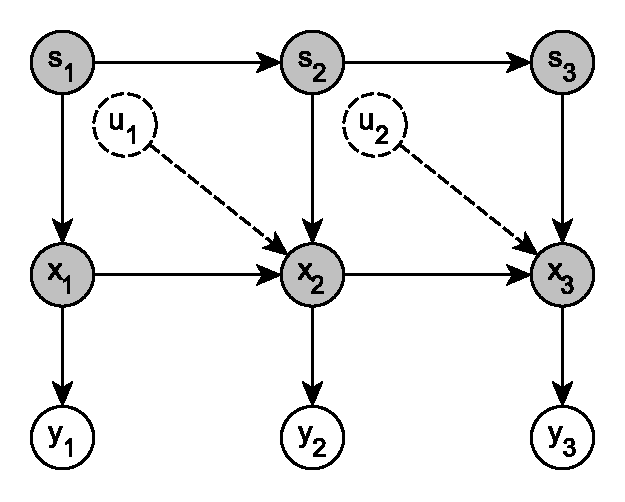
\includegraphics[scale=1.0]{hybrid_model.pdf}
\caption{Graphical model of this section}
\label{fig_hybridmod2}
\end{figure}
Intuitively we are now using the switching variables to decide which nonlinear model better describes the observed system behaviour. At each time point we desire a weighted set of nonlinear models with the weight proportional to the ability of the model to explain the plant behaviour. Such a system could be used to describe significant model changes e.g. catalyst degradation in our CSTR or a reactor which breaks suddenly etc... 

We model this system as follows. Let $s_t=1,2,..., N$ denote a discrete, time homogeneous $N$ state first order Markov chain with transition matrix $P$ as discussed in the previous section. Let each state $s_t=i$ be associated with a model set $\left(f_i, g_i, Q_i, R_i \right)$ used to evaluate the dynamical model shown in (\ref{eq_smodel}).
\begin{equation}
\begin{aligned}
x_{t+1} &= f_i(x_t, u_t, w_{t+1}) \text{ with } w_{t+1} \backsim \mathcal{N}(0, Q_i)\\
y_{t+1} &= g_i(x_{t+1}, v_{t+1}) \text{ with } v_{t+1} \backsim \mathcal{N}(0,R_i)
\end{aligned}
\label{eq_smodel}
\end{equation}
In this dissertation we assume that the the noise distributions are Gaussian but there is no fundamental reason why they cannot be arbitrary. To fully specify the system we again require the prior distributions $p(s_1)$ and $p(x_1|s_1)$.

\subsection{Exact Inference}
By extending the model to incorporate nonlinear models it becomes even more difficult to perform inference. It is clear that for the type of systems we consider here no exact inference algorithm which is computationally feasible exists. We again turn to approximate inference algorithms.

Note that we cannot apply Rao-Blackwellisation as before because the dynamic models are no longer linear. We use the adaptive Sequential Importance Resampling (i.e. the bootstrap) Particle Filter algorithm as discussed in the Nonlinear Models section.

\subsection{Approximate Inference}
We cannot analytically evaluate any part of the desired posterior distribution $p(s_{1:t}, x_{1:t}|y_{1:t})$ so we must apply the adaptive Sequential Importance Resampling algorithm to the entire state space of Figure \ref{fig_hybridmod2}. The algorithm follows straightforwardly from our previous discussion. We merely state the incremental weight function and proposal distribution we sample from in (\ref{eq_nonpf}). 
\begin{equation}
\begin{aligned}
&q_t(s_t,x_t|s_{1:t-1},x_{1:t-1,}y_{1:t}) = p(s_t|s_{t-1})p(x_t|s_t,x_{t-1}) \\
&\alpha_t(s_{1:t},x_{1:t}) = p(y_t|x_t,s_t)
\end{aligned}
\label{eq_nonpf}
\end{equation}  
Applying the algorithm is a straightforward extension of the bootstrap filter shown in the Nonlinear Models section given the weighting function and proposal distribution as shown below.

\textbf{Switching Particle Filter Algorithm}\\
For $t=1$:
\begin{enumerate}
\item
Sample $S^i_1 \backsim p(s_1)$ and $X^i_1 \backsim p(x_1|s_1)$.
\item
Compute the weights $w_1(S_1^i, X_1^i) = p(Y^*_1|S_1^i, X_1^i)$ where $Y^*_1$ is the observation. Normalise $W^i_1 \propto w_1(S_1^i, X_1^i)$. 
\item
If the number of effective particles is below some threshold apply resampling with roughening $(W^i_1, S^i_1, X^i_1)$ to obtain $N$ equally weighted particles $(\frac{1}{N}, \bar{S}^i_1, \bar{X}^i_1)$ and set $(\bar{W}^i_1, \bar{S}^i_1,\bar{X}^i_1) \leftarrow (\frac{1}{N}, \bar{S}^i_1, \bar{X}^i_1)$ otherwise set $(\bar{W}^i_1,\bar{S}^i_1, \bar{X}^i_1) \leftarrow ({W}^i_1, S_1^i, {X}^i_1)$
\end{enumerate}
For $t \geq 2$:
\begin{enumerate}
\item
Sample $S^i_t \backsim p(S_t^i|\bar{S}^i_{t-1})$ and $X^i_t \backsim p(X^i_t|S^i_t, \bar{X}^i_{t-1})$.
\item
Compute the weights $\alpha_t(S_t^i, X_t^i) = p(Y^*_t|S_t^i, X_t^i)$ where $Y^*_t$ is the observation. Normalise $W^i_t \propto W^i_{t-1}\alpha_t(S_t^i, X_t^i)$.
\item
If the number of effective particles is below some threshold apply resampling with roughening $(W^i_1, S^i_t, X^i_t)$ to obtain $N$ equally weighted particles $(\frac{1}{N}, \bar{S}^i_t, \bar{X}^i_t)$ and set $(\bar{W}^i_t, \bar{S}^i_t,\bar{X}^i_t) \leftarrow (\frac{1}{N}, \bar{S}^i_t, \bar{X}^i_t)$ otherwise set $(\bar{W}^i_t,\bar{S}^i_t, \bar{X}^i_t) \leftarrow ({W}^i_t, S_t^i, {X}^i_t)$
\end{enumerate} 

\subsection{Filtering the CSTR}

\subsection{Controlling the CSTR}

\bibliographystyle{plain}
\bibliography{research}

\end{document}